\documentclass[11pt,a4paper]{article}
\usepackage[margin=1in]{geometry}
\usepackage{amsmath,amssymb}
\usepackage{graphicx}
\usepackage{xcolor}
\usepackage{tcolorbox}
\usepackage{listings}
\usepackage{hyperref}
\usepackage{enumitem}
\usepackage{tikz}
\usepackage{array}
\usepackage{multirow}
\usepackage{booktabs}
\usetikzlibrary{shapes,arrows,positioning}

% Define colors for boxes
\definecolor{checkpointcolor}{RGB}{255,223,128}
\definecolor{prereqcolor}{RGB}{173,216,230}
\definecolor{misconceptioncolor}{RGB}{255,182,193}
\definecolor{intuitioncolor}{RGB}{221,160,221}
\definecolor{realworldcolor}{RGB}{255,218,185}
\definecolor{discoverycolor}{RGB}{152,251,152}

% Custom command for conditional probability
\newcommand{\given}{\mid}

% Define custom boxes
\newtcolorbox{checkpoint}{
    colback=checkpointcolor!10,
    colframe=checkpointcolor!80,
    title={\textbf{Checkpoint}},
    fonttitle=\bfseries
}

\newtcolorbox{prereq}{
    colback=prereqcolor!10,
    colframe=prereqcolor!80,
    title={\textbf{Prerequisite Knowledge}},
    fonttitle=\bfseries
}

\newtcolorbox{discovery}{
    colback=discoverycolor!10,
    colframe=discoverycolor!80,
    title={\textbf{Discovery Activity}},
    fonttitle=\bfseries
}

\newtcolorbox{reflection}{
    colback=intuitioncolor!10,
    colframe=intuitioncolor!80,
    title={\textbf{Reflection}},
    fonttitle=\bfseries
}

\newtcolorbox{yourwork}{
    colback=white,
    colframe=gray!60,
    title={\textbf{Your Work}},
    fonttitle=\bfseries,
    boxsep=5mm
}

% Python code style
\lstset{
    language=Python,
    basicstyle=\ttfamily\small,
    keywordstyle=\color{blue},
    commentstyle=\color{green!50!black},
    stringstyle=\color{red},
    showstringspaces=false,
    numbers=left,
    numberstyle=\tiny,
    stepnumber=1,
    frame=single,
    breaklines=true
}

\title{\textbf{Discovering Word Embeddings}\\
\large A Pre-Class Exploration Activity\\
\normalsize Natural Language Processing Course}
\author{Name: \underline{\hspace{5cm}} \quad Date: \underline{\hspace{3cm}}}
\date{}

\begin{document}

\maketitle

\section*{Learning Objectives}
By the end of this discovery session, you will:
\begin{itemize}[leftmargin=*]
    \item Understand why computers need numerical representations of words
    \item Discover the limitations of simple encoding methods
    \item Explore how word meanings can be captured in vectors
    \item Experience the ``magic'' of word arithmetic
    \item Recognize the importance of context in word meaning
\end{itemize}

\begin{prereq}
\textbf{Before starting, you should know:}
\begin{itemize}
    \item Basic Python programming (lists, loops, functions)
    \item What a vector is (a list of numbers)
    \item How to calculate distance between two points
\end{itemize}
\end{prereq}

\vspace{0.5cm}

%==============================================================================
\section{Activity 1: The Word Similarity Challenge}
%==============================================================================

\begin{discovery}
\textbf{Part A: Human Intuition}\\
Rate the similarity between these word pairs on a scale from 0 (completely unrelated) to 10 (identical meaning):

\begin{center}
\begin{tabular}{|l|c|c|c|}
\hline
\textbf{Word 1} & \textbf{Word 2} & \textbf{Your Rating (0-10)} & \textbf{Why this rating?} \\
\hline
cat & dog & \underline{\hspace{2cm}} & \underline{\hspace{4cm}} \\
\hline
cat & kitten & \underline{\hspace{2cm}} & \underline{\hspace{4cm}} \\
\hline
cat & car & \underline{\hspace{2cm}} & \underline{\hspace{4cm}} \\
\hline
king & queen & \underline{\hspace{2cm}} & \underline{\hspace{4cm}} \\
\hline
king & man & \underline{\hspace{2cm}} & \underline{\hspace{4cm}} \\
\hline
happy & joyful & \underline{\hspace{2cm}} & \underline{\hspace{4cm}} \\
\hline
happy & sad & \underline{\hspace{2cm}} & \underline{\hspace{4cm}} \\
\hline
\end{tabular}
\end{center}

\textbf{Part B: The Computer's Problem}\\
If a computer only sees words as strings of characters, how would it calculate similarity?

\begin{lstlisting}
# String comparison - character by character
word1 = "cat"
word2 = "dog"
word3 = "car"

# Count matching characters in same positions
def string_similarity(w1, w2):
    matches = sum(1 for c1, c2 in zip(w1, w2) if c1 == c2)
    return matches / max(len(w1), len(w2))

print(f"cat vs dog: {string_similarity('cat', 'dog')}")
print(f"cat vs car: {string_similarity('cat', 'car')}")
\end{lstlisting}

Run this code and write the results:
\begin{itemize}
    \item cat vs dog: \underline{\hspace{2cm}}
    \item cat vs car: \underline{\hspace{2cm}}
\end{itemize}
\end{discovery}

\begin{reflection}
What's wrong with using character similarity to measure word meaning similarity?

\begin{yourwork}
\vspace{3cm}
\end{yourwork}
\end{reflection}

%==============================================================================
\section{Activity 2: One-Hot Encoding Exploration}
%==============================================================================

\begin{discovery}
\textbf{Part A: Creating One-Hot Vectors}\\
Let's encode words using the one-hot method. Given vocabulary: [cat, dog, mat, sat, hat]

Fill in the one-hot vectors:
\begin{center}
\begin{tabular}{|l|c|c|c|c|c|}
\hline
\textbf{Word} & \multicolumn{5}{c|}{\textbf{One-Hot Vector}} \\
\hline
cat & 1 & 0 & 0 & 0 & 0 \\
\hline
dog & \underline{\hspace{0.5cm}} & \underline{\hspace{0.5cm}} & \underline{\hspace{0.5cm}} & \underline{\hspace{0.5cm}} & \underline{\hspace{0.5cm}} \\
\hline
mat & \underline{\hspace{0.5cm}} & \underline{\hspace{0.5cm}} & \underline{\hspace{0.5cm}} & \underline{\hspace{0.5cm}} & \underline{\hspace{0.5cm}} \\
\hline
sat & \underline{\hspace{0.5cm}} & \underline{\hspace{0.5cm}} & \underline{\hspace{0.5cm}} & \underline{\hspace{0.5cm}} & \underline{\hspace{0.5cm}} \\
\hline
hat & \underline{\hspace{0.5cm}} & \underline{\hspace{0.5cm}} & \underline{\hspace{0.5cm}} & \underline{\hspace{0.5cm}} & \underline{\hspace{0.5cm}} \\
\hline
\end{tabular}
\end{center}

\textbf{Part B: Calculating Similarity}\\
Calculate the dot product (similarity) between vectors:

\begin{lstlisting}
import numpy as np

# Your one-hot vectors from above
cat = [1, 0, 0, 0, 0]
dog = [0, 1, 0, 0, 0]  # Fill in your vector
mat = [0, 0, 1, 0, 0]  # Fill in your vector

# Calculate dot product (similarity)
similarity_cat_dog = np.dot(cat, dog)
similarity_cat_mat = np.dot(cat, mat)

print(f"Similarity(cat, dog) = {similarity_cat_dog}")
print(f"Similarity(cat, mat) = {similarity_cat_mat}")
\end{lstlisting}

Results:
\begin{itemize}
    \item Similarity(cat, dog) = \underline{\hspace{2cm}}
    \item Similarity(cat, mat) = \underline{\hspace{2cm}}
\end{itemize}
\end{discovery}

\begin{checkpoint}
What do you notice about ALL similarity scores with one-hot encoding?

\begin{yourwork}
\vspace{2cm}
\end{yourwork}

If we had 50,000 words in our vocabulary, how many dimensions would each one-hot vector have?
Answer: \underline{\hspace{2cm}}

What percentage of each vector would be zeros? \underline{\hspace{2cm}}
\end{checkpoint}

%==============================================================================
\section{Activity 3: Dense Vectors Discovery}
%==============================================================================

\begin{discovery}
\textbf{Part A: 2D Word Space}\\
Imagine we represent each word with just 2 numbers [x, y] instead of thousands of zeros and ones.

Plot these words on the coordinate system below:
\begin{itemize}
    \item cat = [2, 3]
    \item dog = [3, 3]
    \item kitten = [1.5, 2.5]
    \item car = [8, 1]
    \item truck = [9, 1.5]
\end{itemize}

\begin{center}
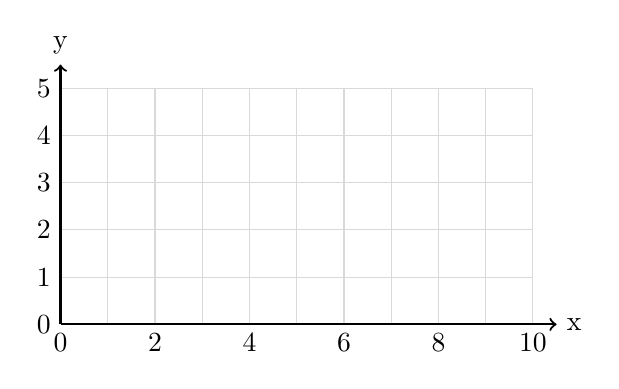
\begin{tikzpicture}[scale=0.6]
    % Draw grid
    \draw[gray!30] (0,0) grid (10,5);
    % Draw axes
    \draw[thick,->] (0,0) -- (10.5,0) node[right] {x};
    \draw[thick,->] (0,0) -- (0,5.5) node[above] {y};
    % Numbers on axes
    \foreach \x in {0,2,4,6,8,10}
        \node[below] at (\x,0) {\x};
    \foreach \y in {0,1,2,3,4,5}
        \node[left] at (0,\y) {\y};
\end{tikzpicture}
\end{center}

\textbf{Part B: Calculate Distances}\\
Use the Euclidean distance formula: $d = \sqrt{(x_2-x_1)^2 + (y_2-y_1)^2}$

\begin{center}
\begin{tabular}{|l|l|c|}
\hline
\textbf{Word Pair} & \textbf{Calculation} & \textbf{Distance} \\
\hline
cat - dog & $\sqrt{(3-2)^2 + (3-3)^2}$ & \underline{\hspace{2cm}} \\
\hline
cat - kitten & \underline{\hspace{4cm}} & \underline{\hspace{2cm}} \\
\hline
cat - car & \underline{\hspace{4cm}} & \underline{\hspace{2cm}} \\
\hline
car - truck & \underline{\hspace{4cm}} & \underline{\hspace{2cm}} \\
\hline
\end{tabular}
\end{center}
\end{discovery}

\begin{reflection}
How do the distances relate to the semantic similarities you assigned in Activity 1?

\begin{yourwork}
\vspace{3cm}
\end{yourwork}

What pattern do you notice about similar words in the vector space?

\begin{yourwork}
\vspace{2cm}
\end{yourwork}
\end{reflection}

%==============================================================================
\section{Activity 4: Word Arithmetic Magic}
%==============================================================================

\begin{discovery}
\textbf{The Famous Example}\\
Word embeddings can capture relationships through vector arithmetic!

Given these simplified 2D vectors:
\begin{itemize}
    \item king = [5, 3]
    \item man = [4, 2]
    \item woman = [4, 1]
    \item queen = [?, ?]
\end{itemize}

\textbf{Part A: Predict the Pattern}\\
If the relationship ``king is to queen as man is to woman'', then:
$$\text{king} - \text{man} + \text{woman} = \text{queen}$$

Calculate step by step:
\begin{enumerate}
    \item king - man = [5, 3] - [4, 2] = [\underline{\hspace{1cm}}, \underline{\hspace{1cm}}]
    \item Result + woman = [\underline{\hspace{1cm}}, \underline{\hspace{1cm}}] + [4, 1] = [\underline{\hspace{1cm}}, \underline{\hspace{1cm}}]
\end{enumerate}

So queen should be approximately: [\underline{\hspace{1cm}}, \underline{\hspace{1cm}}]

\textbf{Part B: Try Your Own}\\
Given:
\begin{itemize}
    \item Paris = [2, 5]
    \item France = [3, 6]
    \item Germany = [7, 6]
\end{itemize}

Predict: Paris - France + Germany = ? (This should give us the capital of Germany)

Your calculation:
\begin{yourwork}
\vspace{3cm}
\end{yourwork}

What real city would this represent? \underline{\hspace{3cm}}
\end{discovery}

\begin{checkpoint}
What does this word arithmetic tell us about how embeddings capture meaning?

\begin{yourwork}
\vspace{3cm}
\end{yourwork}
\end{checkpoint}

%==============================================================================
\section{Activity 5: Context Matters}
%==============================================================================

\begin{discovery}
\textbf{The Problem with Fixed Vectors}\\
Consider the word ``bank'' in these sentences:
\begin{enumerate}
    \item ``I deposited money in the \textbf{bank}.''
    \item ``We had a picnic by the river \textbf{bank}.''
\end{enumerate}

If ``bank'' has a single fixed vector [x, y], answer:
\begin{itemize}
    \item Should ``bank'' be close to ``money''? \underline{\hspace{2cm}}
    \item Should ``bank'' be close to ``river''? \underline{\hspace{2cm}}
    \item Can a single vector satisfy both? \underline{\hspace{2cm}}
\end{itemize}

\textbf{Part B: Dynamic Embeddings}\\
Modern systems (like BERT) create different vectors based on context.

Design two different vectors for ``bank'':
\begin{itemize}
    \item bank (financial) = [\underline{\hspace{1cm}}, \underline{\hspace{1cm}}] (make it close to money=[8,8])
    \item bank (river) = [\underline{\hspace{1cm}}, \underline{\hspace{1cm}}] (make it close to river=[2,2])
\end{itemize}
\end{discovery}

\begin{reflection}
Why are context-dependent embeddings revolutionary for NLP?

\begin{yourwork}
\vspace{3cm}
\end{yourwork}
\end{reflection}

%==============================================================================
\section{Synthesis: Bringing It All Together}
%==============================================================================

\begin{checkpoint}
Based on your discoveries, complete this summary:

\begin{enumerate}
    \item \textbf{Why can't computers use words directly?}
    \begin{yourwork}
    \vspace{2cm}
    \end{yourwork}

    \item \textbf{What's wrong with one-hot encoding?}
    \begin{yourwork}
    \vspace{2cm}
    \end{yourwork}

    \item \textbf{How do dense embeddings solve these problems?}
    \begin{yourwork}
    \vspace{2cm}
    \end{yourwork}

    \item \textbf{What ``magical'' property do good embeddings have?}
    \begin{yourwork}
    \vspace{2cm}
    \end{yourwork}

    \item \textbf{Why do we need contextual embeddings?}
    \begin{yourwork}
    \vspace{2cm}
    \end{yourwork}
\end{enumerate}
\end{checkpoint}

%==============================================================================
\section{Preparation for Class}
%==============================================================================

\textbf{Questions to Ponder:}
\begin{enumerate}
    \item How might a computer \textit{learn} good word vectors automatically from text?
    \item If English has 170,000+ words, how many dimensions should embeddings have?
    \item Could we use embeddings for languages other than English? For emojis? For DNA sequences?
\end{enumerate}

\textbf{Bring to Class:}
\begin{itemize}
    \item This completed handout
    \item Your questions about embeddings
    \item Ideas for applications where embeddings might be useful
\end{itemize}

\vspace{1cm}
\begin{tcolorbox}[colback=blue!5,colframe=blue!40,title={\textbf{Note to Students}}]
This discovery session introduced you to the fundamental concepts of word embeddings. In class, we'll explore how these embeddings are actually learned from data using techniques like Word2Vec and how modern transformer models create contextual embeddings. Your discoveries today form the foundation for understanding these advanced techniques!
\end{tcolorbox}

\end{document}